\documentclass[11pt]{article}
\usepackage{amsmath,amssymb,amsfonts,amsthm}
\newcommand{\numpy}{{\tt numpy}}    % tt font for numpy
\usepackage{graphicx}
\usepackage{xcolor}
\usepackage{listings}
\usepackage[colorlinks = true,
            linkcolor = blue,
            urlcolor  = blue,
            citecolor = blue,
            anchorcolor = blue]{hyperref}
\lstset{basicstyle=\ttfamily\footnotesize,breaklines=true}

\definecolor{mGreen}{rgb}{0,0.6,0}
\definecolor{mGray}{rgb}{0.5,0.5,0.5}
\definecolor{mPurple}{rgb}{0.58,0,0.82}
\definecolor{backgroundColour}{rgb}{0.95,0.95,0.92}

\lstdefinestyle{CStyle}{
    backgroundcolor=\color{backgroundColour},   
    commentstyle=\color{mGreen},
    keywordstyle=\color{magenta},
    numberstyle=\tiny\color{mGray},
    stringstyle=\color{mPurple},
    basicstyle=\ttfamily\footnotesize,
    breakatwhitespace=false,         
    breaklines=true,                 
    captionpos=b,                    
    keepspaces=true,                 
    numbers=left,                    
    numbersep=5pt,                  
    showspaces=false,                
    showstringspaces=false,
    showtabs=false,                  
    tabsize=2,
    language=C
}


\topmargin -.5in
\textheight 9in
\oddsidemargin -.25in
\evensidemargin -.25in
\textwidth 7in

\begin{document}
% ========== Edit your name here
\author{Yida Liu, Charles Novitsky, Chang Deng}
\title{EECS 444 Homework 1 Part 2}
\maketitle

\section{Crack the password}

\subsection{Zip Password}

% Here we used brute force method for resolving the password for the \lstinline{ .zip} file. We noticed that the password is only a combination of 1-2 words from the word list, numbers and two special character, \@ and \$. The cracking is not as hard as it might seem to be: it took about an hour and 15 minutes in an laptop with 2 cores and 8 Gib memory with power-saver mode on. The password for file \lstinline{Group A_CYBE_HW1-P2_64bit.zip} is \lstinline{5@Paris\$}.

% The source code can be found on \href{https://github.com/Mestrace/EECS444-Computer-Security/blob/master/Assignment/1/Part2/crack\%20zip.ipynb}{this IPython notebook} on Github

\begin{enumerate}
    \item Is the word less than 5 letter? \par
    No
    \item Is there more than 1 number? \par
    No, there is only 1 number.
    \item Is the number odd? \par
    Yes.
    \item Does the word has a 'P'? \par
    Yes. Eliminate down to 'Paris' and 'Puppy'
    \item Is most of the word in the second half of the password?\par
    Yes.
    \item Does the password start with a number? \par
    No
    \item Are they the same special character? \par
    No
    \item Is the number greater than 5? \par
    No. Could be 1, 3, 5.
    \item Does the dollar sign come before the at sign??
    No.
    \item Is the dollar sign the last character? \par
    Yes. 
\end{enumerate}

This eliminates our guess on $\#@W\$$, where \# is a number in $[1, 3, 5]$, $W$ is a word in $[\text{Puppy, Paris}]$, which gives us only 6 choices. We tried a few combinations, and found out that the password to the .zip file is $\text{5@Paris\$}$.

\subsection{System Password}\label{syspw}

After we open the program, \lstinline{CYBE_HW1-P2_64bit.exe}, we were prompted to enter a password for system entry. At the first attempt, we tried inputting a relatively long string for the password. To be specific, we entered 257 "a"s. This does not work out. This suggest that the input buffer is a large one. 

The program prints exactly the string we entered. This might be a loop hole. Therefore, we changed our mind by using the string formatting attack with \lstinline{\%x}. Our assumption is that, if the password-input buffer and the actual-password buffer are closely defined, their relative location on the stack will be close. As sufficient \lstinline{\%x} is supplied, the program will print the stack values which contains the actual password. Our 2nd attempt worked out. We put 35 \lstinline{\%x}s and the program output is
\begin{lstlisting}
d8da5940 62f958 70 61 73 73 77 72 6f 73 64 3a 43 53 24 34 39 33 5e 32 30 31 38 2d 30 32 2d 30 31 0 0 0 0 0 408ba0 402460 400000 is not the password
\end{lstlisting}
The suspicious numbers in the middle could be decoded to ASCII string \lstinline{passwrosd:CS\$493^2018-02-01}. Fortunately, the password to the ticket system is exactly the string after the colon \lstinline{CS\$493^2018-02-01}, notwithstanding the misspelled "password". 

\section{Purchase the ticket}\label{purticket}

On the next screen, we were prompted to purchase a 500-dolloar ticket with \$480 balance in the account. Although we cannot buy 1 ticket with the \$480, dollars, we utilized the arithmetic overflow of the \lstinline{unsigned short} data type for storing the subtotal price to purchase -131 tickets and we were able to get the ticket for only \$36.

\section{Upgrade the seat}\label{seatup}

Lastly, we were prompted to enter the customer information for the person taking planes. We thought that if the class is stored in some buffer, it is possible that we could use buffer overflow to over-write the class information. Notice that the d.o.b is right before the class information when printed, after a few trial, we entered \lstinline{09/08/1996      First} (notice the 6 spaces) as our d.o.b and successfully obtain the following print-out:
\begin{center}
\begin{tabular}{c}
\begin{lstlisting}
--------ticket 5 info-------------
Name:Liu,Yida
Date of birth:09/08/1996
Class:First
----------------------------------
\end{lstlisting}
\end{tabular}
\end{center}
, which upgraded the class to first.

\appendix
\section{Screenshots}
\subsection{System Password}
The screenshot to the Section \ref{syspw}, System Password. 
\begin{center}
    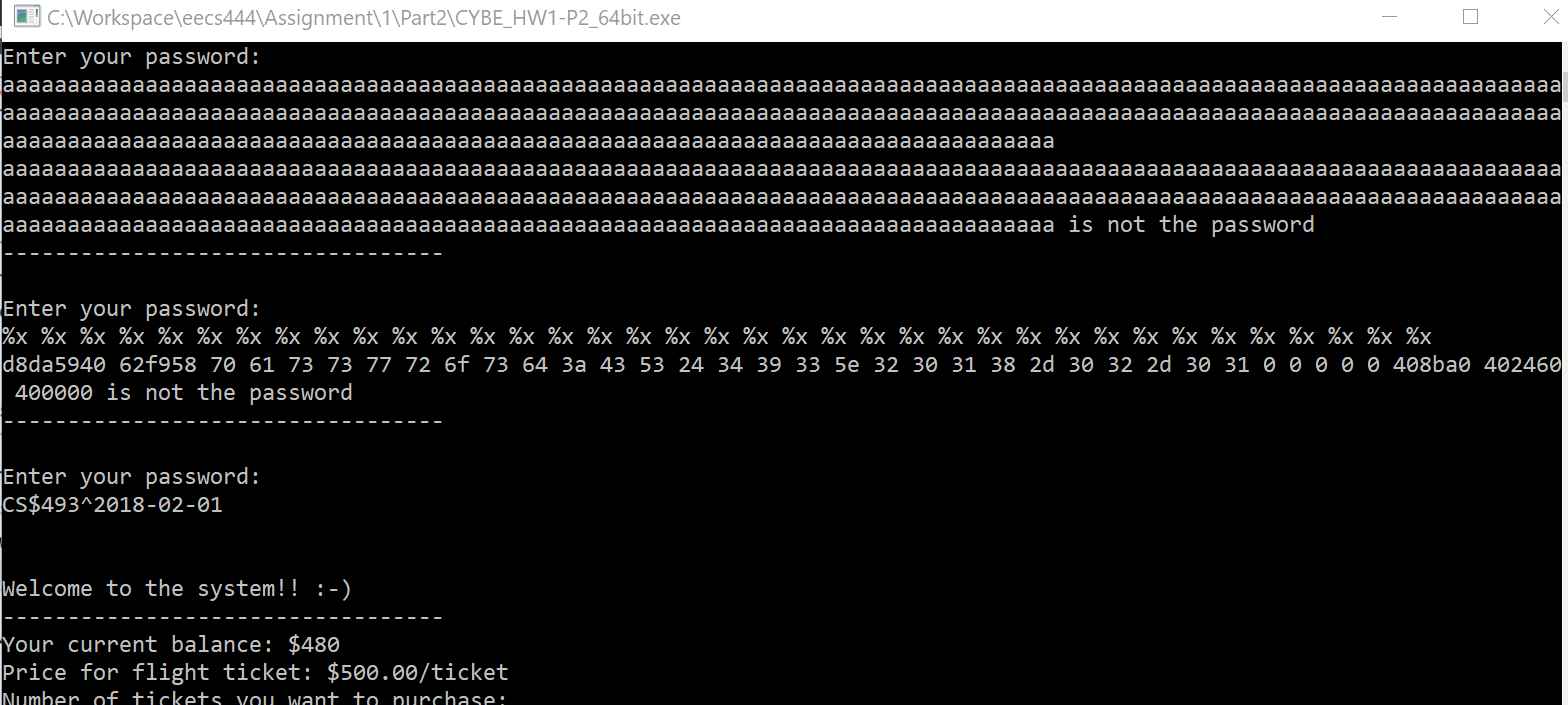
\includegraphics[width=\textwidth,scale=0.5]{{Assignment/1/Part2/p2q1s2.png}}
\end{center}

\clearpage
\subsection{Purchase the Ticket}
The screenshot to the Section \ref{purticket}, Purchase the Ticket.
\begin{center}
    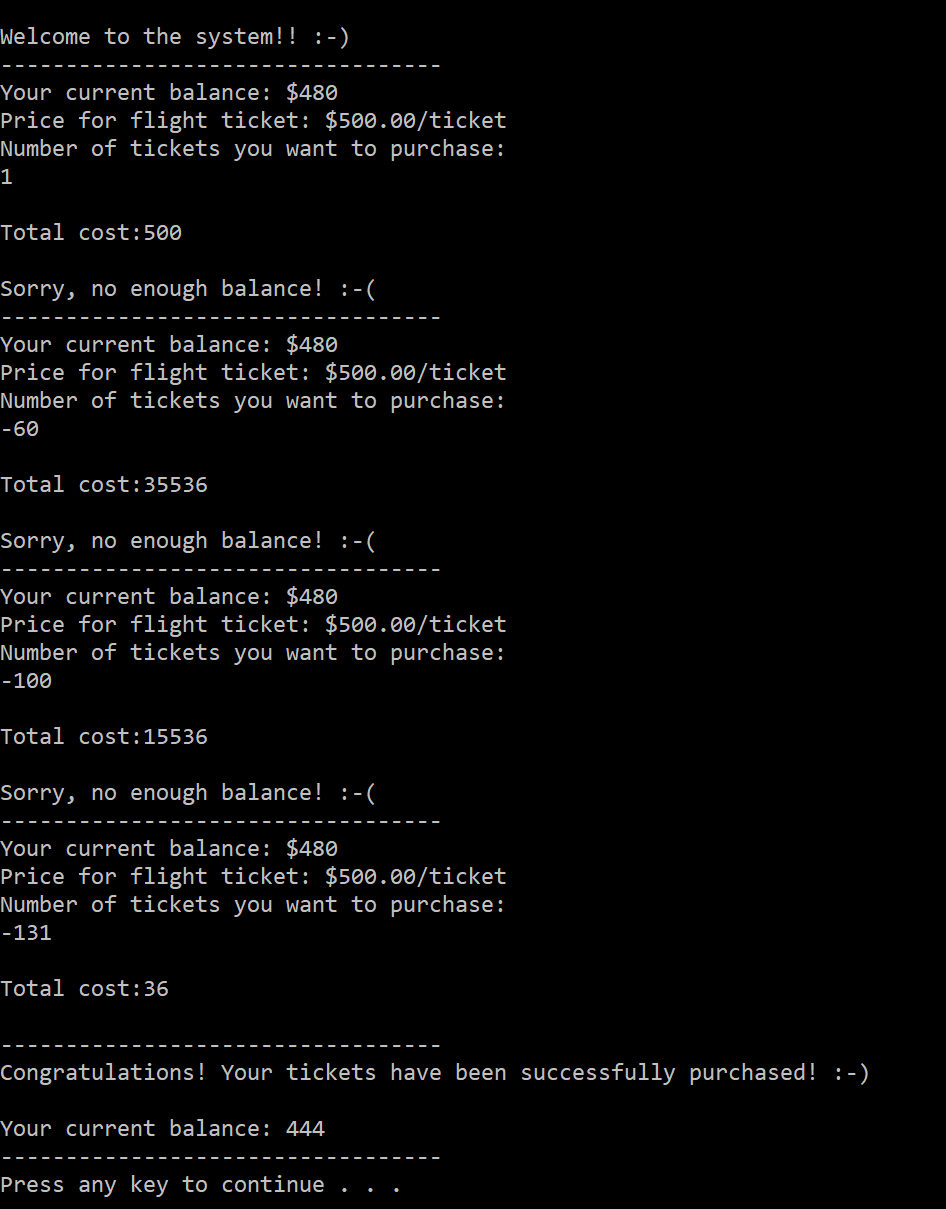
\includegraphics[scale=1]{{Assignment/1/Part2/p2q2.png}}
\end{center}

\clearpage
\subsection{Upgrade the Seat}
The screenshot to the Section \ref{seatup}, Upgrade the seat.

\begin{center}
    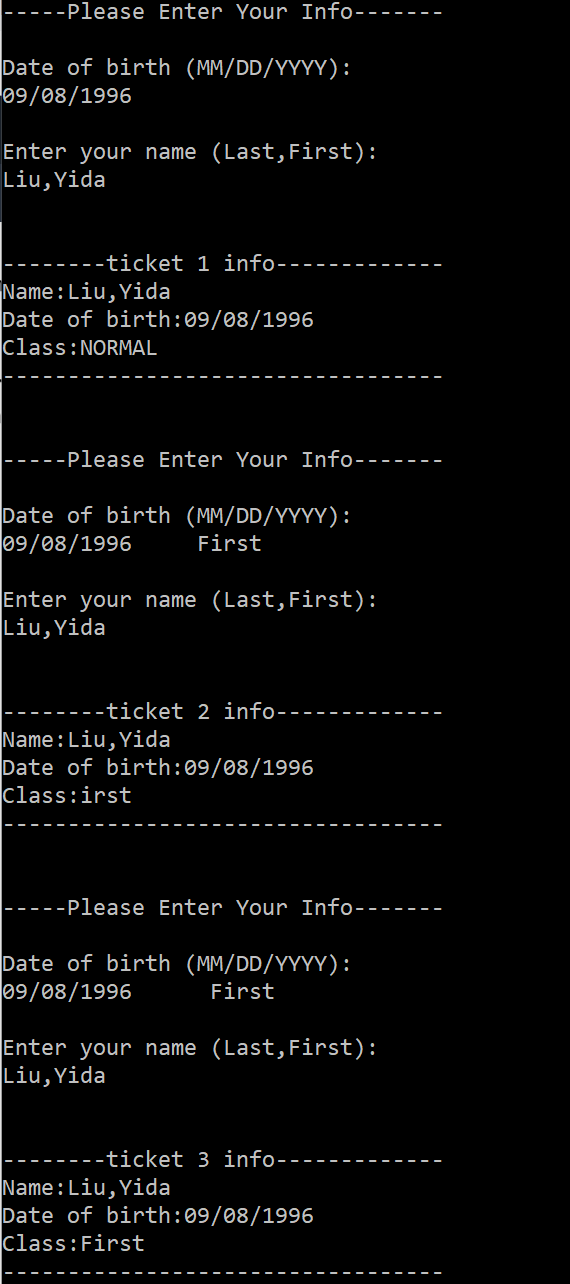
\includegraphics[scale=1.1]{{Assignment/1/Part2/p2q3.png}}
\end{center}
\end{document}